\section{Introduction} 

%% TODO - repeated whole cloth from the abstract
Nearly all current technologies for applying force and torque between two spacecraft share a disadvantage: they require either propellant or mechanical contact. By using the force between a magnetic field and the electric currents it induces in a conductive target, a new technology known as an induction coupler exploits eddy-current effects to control the relative position and orientation between a chaser spacecraft and a target without mechanical contact. The induction coupler does not rely on familiar magnetic attraction and repulsion, which would require ferromagnetic materials on the target.  In contrast, and induction coupler is broadly applicable for even uncooperative targets, as long as the target includes conductive materials, as is generally the case for spacecraft.[1]

An induction coupler creates actuation force by producing a time-varying magnetic that induces eddy-currents  through the conductive materials in a target. The coupler’s magnetic field then exerts a force on these currents and thus the target. The coupler requires no mechanical contact with a target, nor does it demand cooperation from the target. The coupler operates on electricity alone, enabling close-proximity navigation without propellant. Because most satellites include conductive material in their structure—notably aluminum honeycomb with aluminum facesheets, aluminum isogrid, and aluminum truss elements—induction couplers may be the closest thing we have to science fiction's tractor beam: a device that can produce contactless force on an uncooperative target. It can also be thought of as a contactless momentum-transfer actuator.

Induction couplers show promise for spaceflight applications, offering three major advantages. First, the force associated with magnetic fields across meter-scale distances can dominate gravity, aerodynamic drag, and other effects, which are far less pronounced in orbit than in a terrestrial environment. Second, fully deployed spacecraft are fragile and rarely offer straightforward means for mechanical grappling; so, the ability to interact without the potential for contact damage is valuable. Third, induction couplers offer the ability to maneuver without propellant, eliminating risks associated with thruster-plume impingement \cite{BaerwaldR.S.1977}
and extending the useable lifetime of the chaser spacecraft.
A small spacecraft could use induction couplers to control its motion relative to a much larger target like the International Space Station (ISS), crawling just above the target’s surface without ever touching. This on-orbit inspection technique resembles the operations concept for underwater robots that now inspect pipelines and shipwrecks. \cite{Whitcomb2000}

\begin{figure}
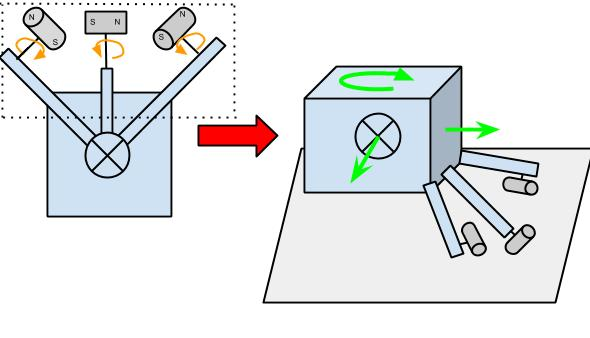
\includegraphics[width = 4cm, height = 4cm ]{figures/Induction_Coupler_Overview_Diagram.jpg}
\label{fig:inspector_diagram}
\caption{A spacecraft can use an induction coupler with three spinning magnets to create actuation force and torque}
\end{figure}
 
Current interest in on-orbit servicing (OOS) is a strong motivation for advancing induction coupler technology. \cite{Ambrose2012}
 One of the more compelling use cases is that of a small inspection vehicle whose interactions with the target do not produce significant motion in that target—for example, an ISS inspection vehicle. Such a vehicle is primarily concerned with regulating planar motion along the surface of the target and stabilization of out-of-plane translation. This paper describes a study of how the in-plane component of that motion can be achieved with induction couplers.


